%!TeX root = thesis-main.tex
%basicstyle=\fontsize{8}{9}\selectfont\ttfamily

%%%%%%% %%%%%%%%  %%%%%%% 
%%%%%%% COMMANDS  %%%%%%%
%%%%%%% %%%%%%%%  %%%%%%%


\sloppypar

%\chapter{Towards Reinforcement Learning-based Aggregate Computing}
\chapter[Collective Program Sketching]{Program Sketching with Aggregate Computing}\label{chap:learning:sketching}%\mtcaddchapter
\minitoc% Creating an actual minitoc
\begin{comment}
The pervasiveness of computing and networking
 fosters applications 
 backed by large-scale cyber-physical collectives---cf. edge-fog-cloud infrastructures, robot swarms, %power grids, 
 and smart ecosystems.
%
Combined with the \emph{autonomic computing} vision ~\cite{DBLP:journals/computer/KephartC03}, which promotes autonomy and self-* capabilities in engineered systems,
 there is an increasing trend towards \acp{cas} and their engineering~\cite{DBLP:journals/sttt/NicolaJW20,DBLP:journals/tasm/BucchiaroneDPCS20}.
%
\acp{cas} are characterized 
 by a multitude of agents  
 that can produce globally coherent results (\emph{emergents}~\cite{DBLP:conf/atal/WolfH04}),
 and collective-level adaptivity to environment change
 via local decision-making and decentralized interaction.
%
The \emph{engineering of \acp{cas}} is an open research problem~\cite{DBLP:journals/sttt/NicolaJW20,DBLP:journals/corr/abs-1108-5643} of significance, tightly linked with the problems of ``steering'' self-organization and ``controlling'' emergence to promote desired while avoiding undesired emergents~\cite{DBLP:books/sp/08/Muller-SchloerS08}.
%
In general, when dealing with \acp{cas},
 there are two distinct problems:
 (i) given an initial system state and local behavioural rules, predicting what global outcomes will be produced (\emph{forward}, \emph{prediction}, or \emph{local-to-global problem});
 and
 (ii) what local behavioural rules must be assigned to the system devices to achieve certain global outcomes (\emph{inverse}, \emph{control}, or \emph{global-to-local problem}).
%
These two problems provide corresponding perspectives
 for \emph{designing} \acp{cas}.
% 
In particular, the latter perspective has promoted research on \emph{spatial} and \emph{macro-programming}~\cite{beal2013organizing-aggregate,DBLP:journals/corr/abs-2201-03473}
 aiming at expressing programs in terms of the desired global outcome
 and leaving the underlying platform to deal with the global-to-local mapping.

In this work,
 we consider \emph{\ac{ac}}~\cite{DBLP:journals/computer/BealPV15}, a prominent \emph{field-based coordination} approach~\cite{DBLP:journals/jlap/ViroliBDACP19} 
promoting macro-programming 
 by capturing \ac{cas} behaviours 
 as functions operating on \emph{computational fields}~\cite{DBLP:journals/jlap/ViroliBDACP19},
 in a system model of neighbour-interacting devices
 operating in asynchronous sense-compute-interact rounds.
%
A computational field is a macro-abstraction
 that maps a set of devices over time to computational values.
%
\ac{ac} is based on the \emph{\ac{fc}}~\cite{DBLP:journals/jlap/ViroliBDACP19}, or variants thereof,
 that define constructs for manipulating and evolving fields.
%
\end{comment}
\ac{cpsw} behaviour
 can be expressed by a single \emph{aggregate program} (global perspective)
 that also defines 
 what processing and communication activities
 must be performed by each individual device (local perspective).

Besides the programming model and its implications,
 a significant portion of research on \ac{ac}~\cite{DBLP:journals/jlap/ViroliBDACP19} has focussed
 on design and analysis of \emph{coordination algorithms} expressed in \ac{fc}
 for efficiently carrying out self-organising behaviours
 like, e.g., computing fields of minimum distances from sources (\emph{gradients})~\cite{DBLP:conf/ipsn/NagpalSB03,DBLP:journals/pervasive/MameiZL04,DBLP:conf/saso/AudritoCDV17},
 electing leaders~\cite{DBLP:conf/saso/MoBD18},
 or %collecting data %on spanning trees 
 %for 
 distributed summarization~\cite{DBLP:journals/cee/AudritoCDPV21}.
%
However, devising self-organising coordination algorithms is not easy; especially difficult is identifying solutions
 that are efficient across environment assumptions, configurations, and perturbations.
%
The difficulty lies in determining, 
 for a current context,
 the local decisions of each device, 
 in terms e.g. of processing steps and communication acts,
 producing output fields that quickly converge to the correct solution.

In chapter we adopt a \emph{\ac{rl}-based approach}---where an agent learns from experience
 how to behave in order to maximize delayed cumulative rewards.
%
We devise a general methodology that somewhat resembles the notion of \emph{sketching} in program synthesis~\cite{solar2008program-synthesis-sketching}:
 a template program is given and \emph{holes} are filled with actions determined through search.
%
In our case, the program is the \ac{ac} specification of a coordination algorithm, and holes are filled with actions of a policy learnt through a multi-agent reinforcement learning algorithm called Hysteretic Q-Learning~\cite{DBLP:conf/iros/MatignonLF07}.
%
We consider the case of the classic gradient algorithm, a paradigmatic and key building block of self-organising coordination \cite{DBLP:journals/jlap/ViroliBDACP19,beal2013organizing-aggregate,DBLP:journals/corr/abs-2201-03473}: we show via simulations 
 that the system, after sufficient training,
 learns an improved way to compute and adjust gradient fields to network perturbations.

\section{On Integrating Machine Learning and Aggregate Computing}
As anticipated in \Cref{part:background}, 
 the behaviour of an aggregate system depends on the interplay of three main ingredients:
\begin{itemize}
  \item the aggregate program, expressing conceptually the global behaviour of the entire system, and concretely the local behaviour of each individual node in terms of local processing and data exchange with neighbours; and
  \item the aggregate execution model, promoting a certain dynamics of the system in terms of topology management (e.g., via neighbour discovery), execution of rounds, scheduling of communications; and
  \item  the environment dynamics.
\end{itemize}
%
While the latter cannot be controlled, 
 the importance of the first element is reflected by research
 on the design of novel algorithms (cf.~\cite{DBLP:journals/jlap/ViroliBDACP19,DBLP:conf/saso/AudritoCDV17}),
 while the second element is studied 
 w.r.t. the possibility of tuning and adaptivity 
 according to 
 available technology and infrastructure 
 or the dynamics of the environment---see the previous chapter. %(e.g. reacting to a phenomenon that changes quickly requires increasing the execution frequency---cf.~\cite{danilo2021lmcs}).
%
Since tuning programs or execution details to specific environments
 or adapting those to changing environments
 can be burdensome,
 it makes sense to consider the use of machine learning techniques
 to let a system \emph{learn} effective strategies for unfolding collective adaptive behaviour.
%

\section{Aggregate Programs Improvement through \ac{rl}}
%!TeX root = thesis-main.tex

\begin{figure}[t]
  \centering
  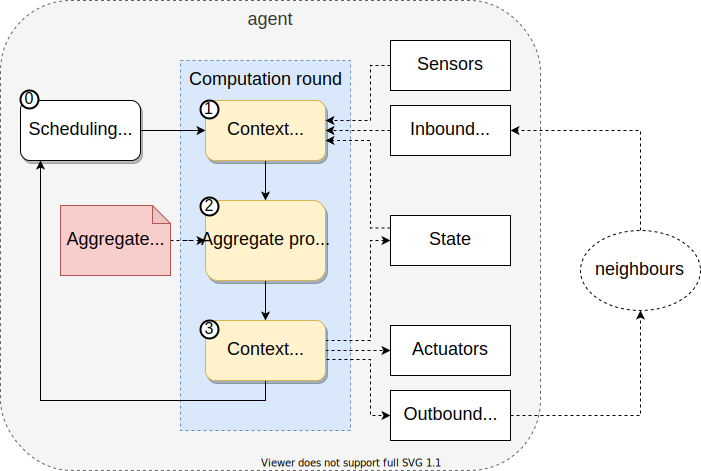
\includegraphics[width=0.9\textwidth]{papers/coordination2022/img/aggregate-agent-control-architecture.pdf}
  \caption[Integration of \ac{RL} within the \ac{ac} control architecture for collective program synthesis]{Integration of \ac{rl} within the \ac{ac} control architecture~\cite{DBLP:journals/jsan/CasadeiAV21}. 
  %
  The \ac{rl} state and reward concepts build upon the context, given by environment and neighbour data. 
  %
  The designer configures action points where learning can improve the aggregate computation. 
  %
  The actions selected by the learned policies will then affect the environment (via actuators) and neighbours (via outbound messages).}
  \label{coordination2022:fig:ac-and-rl}
\end{figure}

In this work, we focus on \emph{improving aggregate programs}
 by learning effective local actions
 within a given algorithmic schema---an approach similar to the \emph{sketching} technique for program synthesis~\cite{solar2008program-synthesis-sketching}.
Differently from the previous chapter, 
 where we used \ac{rl} to improve the execution model, 
 here we use \ac{rl} to improve the aggregate program.
% \meta{TODO: explain why RL and not other ML techniques}.
As a learning framework,
 we use \ac{rl} as 
 we deal with systems of agents 
 performing ongoing activities 
 by interacting with one another and the environment. 
%
Specifically we integrate \ac{rl} within the \ac{ac} control architecture in order to support learning of good collective behaviour sketched by a given aggregate program (\Cref{coordination2022:fig:ac-and-rl}).
%
Specifically, 
 we focus on improving \ac{ac} building blocks (such as the gradient algorithm covered in \Cref{part:background}) through learning, 
 leading toward a so-called \emph{reinforcement learning-based aggregate computing}. 
%
Learning, thus, does not replace the \ac{ac} methodology for defining the programs, 
 but it is best understood as a technique that supports and improves the \ac{ac} algorithm design process. 
\section{Building blocks Refinement}\label{coordination2022:s:learning-gradient}
A major advantage of \ac{ac} as a programming model is its \emph{compositionality}: complex collective behaviours (e.g., the maintenance of a multi-hop connectivity channel) can be expressed through a combination of building blocks capturing simpler collective behaviours (e.g., gradients).
%
Since building blocks are fundamental bricks of behaviour that often recur in programs, 
 their bad and good qualities (cf., convergence speed, stability, etc.) tend to amplify and affect behaviours that depend on them.
%
Therefore, research tends to investigate refined variants of building blocks that provide the same functionality but are more \emph{effective} or \emph{efficient} under specific assumptions or contexts (e.g., high mobility, situations where stability is more important than precision, etc.)~\cite{DBLP:conf/saso/AudritoCDV17,DBLP:journals/cee/AudritoCDPV21}.
%
With a library of algorithms, 
 the designer can choose the best combination of building blocks that are well-fitted for a given environment, 
 and even substitute a building block with a variant implementation without substantially affecting the application logic.
%\meta{@GA to @All, in sec 4.1 I show a gradient block with opt. Probably here we need to show a general structure? With images? }
In general, a building block can be seen as a \emph{black box} (function) that takes a set of input fields (e.g. metric, perception fields, constant fields, etc.) and yields an output field. 
%
To increase its flexibility, 
 such a function could leverage a \emph{refinement policy} able to affect the behaviour of the building block over time or in a certain situation. 
%
This policy could be a feedback loop, hysteresis, or custom logic to solve a specific problem.
%
We aim at structuring the learning of refinement policies through \ac{rl}~\cite{DBLP:conf/acsos/Aguzzi21}.
%
Our idea is that it should not be the designer who codes a particular block to be used, 
 but that it is the learning algorithm that understands, given a global policy to be optimized following a utility function, 
 what actions need to be activated.
% to optimise the collective good of the system.

%!TeX root = paper22-coord-ac-rl.tex
\begin{figure}[t]
  \includegraphics[width=\textwidth]{papers/coordination2022/img/algorithm-learning.pdf}
  \caption[Reinforcement Learning schema used in program synthesis simulations]{
  Reinforcement Learning schema used in our simulations.
  The learning algorithm is applied at simulation time (for $T$ episodes) improving a shared $Q$ table. 
  %
  At the deployment time then, the agents exploit a local copy of the optimal $Q^*$ table found by learning.}
  \label{coordination2022:fig:learning-scheme}
\end{figure}

The continuous and variable state problems are typically tackled using deep learning to learn the right state representation for a given problem~\cite{DBLP:journals/corr/abs-1806-08894}. %and Graph Neural Networks (to regulate variable-size inputs). 
%
In this case, instead, we used a handcraft feature engineering process since we are more interested in devising a general design process.

Concerning the \emph{multi-agent credit assignment problem}, 
we decided to use offline learning 
%based on simulation and then the policy is deployed in a concrete system 
in a typical \ac{ctde} setting (\Cref{coordination2022:fig:learning-scheme}).
%
This way, we assess the influence of an individual in comparison to the entire system, 
which cannot be done in online learning due to the difficulty of achieving global snapshots of the system in a reasonable time.

\section{Learning Schema} 
The learning algorithm is seen as a state ($s_t$) evolution function in which the nodes try to apply a correction factor (\lstinline|update|) following a policy ($\pi^Q_{target}$ or $\pi^Q_{behavioral}$) refined by learning.
%
The state is built from a neighbourhood field of the building block generic output ($o_t$) passed as input.
%
\Cref{coordination2022:lst:general-schema} exemplifies the general program structure used to combine \ac{rl} with \ac{ac} for improving building blocks.
%
The branching operator (\lstinline|branch|) on \lstinline|learn| condition makes it possible to use the \ac{ctde} schema since when the \lstinline|learn| is \lstinline|false| there is no need for a central entity (\lstinline|simulation|).
%
The Q table is gathered using \lstinline|sense|, a \scafi{} operator used to query sensors and collect data from them. 
%
At simulation time, Q is a shared object, 
 but at runtime each agent owns a local table.
%
%!TeX root = paper22-coord-ac-rl.tex

\begin{lstlisting}[
  mathescape,
  %float=tp,
  floatplacement=tbp,
  frame=single,
  label={lst:general-schema},
  caption={
    ScaFi-like pseudocode description (implemented in the simulation) for value-based \ac{rl} algorithm applied \ac{ac}.
    %
    \texttt{state}, \texttt{update}, \texttt{reward} are block specific. 
    %The learn branch use \texttt{simulation}, a global object in which agents access to a shared Q.
  },
  captionpos=b
]
def optBlock($o_{t-1}$) { // learning as a field that evolves in time
  rep(($s_0, a_0$, $o_0$)) { // $s_0$, $a_0$ context dependent 
    case ($s_{t-1}, a_{t-1}$, _) => {
      val Q = sense("Q") // global during training, local during execution
      val $o_{t}$ = update($o_{t-1}$, $a_{t-1}$) // local action
      // state from the neighbourhood field program output
      val $s_{t}$ = state(nbr($o_{t}$))
      val $a_{t}$ = branch(learn) { // actions depends on learn condition
        val $r_{t-1}$ = reward($o_{t}$, simulation) // simulation is a global object
        simulation.updateQ(Q, $s_{t-1}$, $a_{t-1}$, $r_{t-1}$, $s_{t}$) // Q update
        $\sim$ $\pi_{behavioural}^Q$($s_{t}$) // sample from a probabilistic distribution
      } {
        $\pi_{target}^Q$($s_t$) // greedy policy, no sampling is needed
      }
    }
    ($s_{t}$, $a_{t}$, $o_{t}$) 
  }._3 // select the output from the tuple
}
  \end{lstlisting}
  %\caption{\scafi{}-like pseudocode description for value-based \ac{rl} algorithm applied \ac{ac}. \texttt{state}, \texttt{update}, \texttt{reward} are block specific. The learn branch use \texttt{simulation}, a global object in which agents access to a shared Q. 
  %$\sim$ stands for sampling a value from a probabilistic distribution.}
  %\label{lst:general-schema}
%\end{figure}
%
Finally, the produced $o_{t}$ is returned to the caller.

In this case, we encoded the learning process with \ac{ac} itself. 
%
Though we could have extracted the learning process from the \ac{ac} program, %producing a policy usable in \ac{ac},
 we took this decision because: 
\begin{itemize}
  \item it allows us to extend learning by exploiting neighbourhood Q table fields -- so we can think of doing non-homogeneous learning in different areas of the system;
  \item the scheme for taking state and choosing actions is the same as the one we would need for learning, so the only difference is in the branch; and
  \item it can simply be extended to online learning.
\end{itemize}
%
%In the next section, we describe an incarnation of this algorithm applied to the gradient block.

\section{Reinforcement learning-based gradient block}
%\meta{@GA to @All: another way to generalise G?}
The gradient block could be generalized as follows:
\begin{lstlisting}
def gradientOpt(source, metric, opt) {
  rep(infinity) { g => mux(source) { 0 } { opt(g, metric) } }
}
\end{lstlisting}
where \lstinline|opt| is a function that determines how to evolve the gradient based on the field of current gradient values \lstinline|g| and current \lstinline|metric| (estimation of distances to neighbour). 
%In this way, the correction factor applied to the gradient could be composed, creating a gradient block that handles several scenarios.
In this chapter, we examine \lstinline|opt| as an \emph{hole}, 
 a placeholder that a reinforcement learning (\ac{rl}) algorithm fills based on raw experiential interactions. 
 The primary objective is the incremental construction of a gradient field, while also aiming to mitigate the \emph{rising-value} issue. 
 This issue is also known as the \emph{count to infinity} problem in the domain of field-based coordination. 
 It manifests as the system's inefficiency in rapidly responding to an increase in output needs (e.g., when a source node deactivates), 
 despite its proficiency in handling situations requiring a reduction in output (e.g., when a new source is introduced).

The literature provides various heuristic solutions to overcome the limitations of traditional gradient methods~\cite{DBLP:conf/saso/AudritoCDV17}. 
 One notable technique is the Constraint and Restoring Force (CRF)~\cite{DBLP:conf/sac/BealBVT08}, 
 designed to enforce a uniform rate of increase in the gradient field when nodes detect a local, slow ascent. 
 In this context, each node is influenced by a set of constraints, specifically, nodes that possess lower gradient values. 
 If a node identifies a sluggish increase and finds itself unconstrained, it elevates its output at a fixed rate, independent of its neighbors. 
 Otherwise, it adheres to the traditional gradient formula. 
 Our proposed learning algorithm aims to emulate this behavior while eliminating the necessity for manual algorithmic design.

To articulate our learning problem, 
 we employ the general schema depicted in \Cref{coordination2022:fig:learning-scheme}. 
 The \lstinline|state| function captures sufficient information for agents to dynamically accelerate local value increases. 
 Specifically, we define the state \( s_t \) as the difference between a node's perceived output and the minimum and maximum gradient values received from its neighbors: \( s_t = (|min_t - o_t|, |max_t - o_t|) \). 
 To manage the high dimensionality of this state space, we employ discretization, thereby mitigating the risk of overfitting. 
 The discretization is governed by two parameters: 
 \( maxBound \) and \( buckets \). 
 \( maxBound \) constrains the output to a range between \( - radius \times maxBound \) and \( radius \times maxBound \), where \( radius \) is the maximum communication range of the nodes. 
 Values outside this range are considered equivalent states. 
 \( buckets \) defines the granularity of the discretization within this specified range.

To incorporate historical data, 
 we stack the states from two successive time steps to form \( h_t = [(s_{t - 1}, s_t)] \). 
 This composite state \( h_t \) serves as the input state for our \ac{rl} algorithm, 
 resulting in a state space cardinality of \( |s_t| \times |s_t| = buckets^4 \).

The action space is bifurcated into two categories: 
 \texttt{ConsiderNeighbourhood}, 
 which executes the traditional gradient evaluation, and \texttt{Ignore(velocity)}, 
 which disregards neighboring data to adjust the gradient at a designated \texttt{velocity}. 
 The corresponding \texttt{update} function is defined accordingly:
\begin{lstlisting}[mathescape]
def update($o_{t-1}$, $a_{t-1}$, metric) = // $o_{t-1}$ is the previous gradient output
  val $g_{classic}$ = minHoodPlus(nbr($o_{t-1}$) + metric())
  match $a_{t-1}$ // scala-like pattern matching
    case ConsiderNeighbourhood => $g_{classic}$
    case Ignore(velocity) => $o_t$ + velocity * deltaTime() 
\end{lstlisting}
%
Finally, the \texttt{reward} function is described as follows: 
\begin{lstlisting}[mathescape]
def reward($o_t$, simulation) {
  if($o_t$ - simulation.rightValueFor(mid()) $\sim$= 0) { 0 } { -1 }
}
\end{lstlisting}
In this context, the function \lstinline|mid| retrieves the corresponding field of node identifiers. 
 The overarching goal is to compel the nodes to generate output values that closely approximate the ideal gradient values as stipulated by a trusted oracle, represented by the function \lstinline|simulation.rightValuefor()|.

When the output aligns with the expected ideal value, a reward of $0$ is issued. Conversely, if the output diverges from the expected value, 
 a minor punitive measure in the form of a negative reward, $-1$, is administered. This is designed to expedite the nodes' convergence toward a state where the actual output closely mirrors the ideal value.
\section{Evaluation}\label{coordination2022:s:eval}

\begin{table}[t]
  \centering
  \begin{tabular}{|c|c|}
    \hline
    Name &  Values \\ \hline
    $(\gamma)$ & [0.4 -- 0.7 -- 0.9] \\  \hline
    $(\epsilon_0, \theta)$ & [(0.5,200) -- (0.01,1000) -- (0.05,400) -- (0.02,500)] \\ \hline
    $(\beta, \alpha)$ & [(0.5,0.01) -- (0.5,0.1) -- (0.3,0.05) -- (0.2,0.03) -- (0.1,0.01)]
    \\  \hline
    (buckets, maxBound) & [(16,4) -- (32,4) -- (64,4)]\\ \hline
  \end{tabular}
  \caption{Summary of the simulation variables. 
  %
  A simulation is identified by a quadruple $(i, j, k, l)$ of indexes for each variable. 
  %
  %So simulation 0000 is the one with $\gamma = 0.4, \epsilon_0 = 0.5, \theta = 200, \beta = 0.5, \alpha = 0.01, buckets = 16,  maxBound = 4$.
  }
  \label{coordination2022:table:parameters}
\end{table}

To evaluate our approach, we run a set of Alchemist simulated experiments and verify that an aggregate system
 can successfully learn an improved way to compute a gradient field (cf. the gradient block described in \Cref{part:background}).
%
The source code, data, and instructions for running the experiments have been made fully available at a public repository\footnote{\url{https://github.com/cric96/experiment-2022-coordination}}, to promote reproducibility of results.

\subsection{Simulation setup}

The simulation comprises $N$ devices, 
 organized within a structured grid. 
 The grid environments employed for this study fall into two categories, 
 each having identical dimensions with respect to width (\SI{200}{\metre}) and inter-node spacing (\SI{5}{\metre}). 
 However, they differ in the number of rows: 
 the first scenario features a single row (essentially aligning the nodes linearly), while the second includes five rows.

The total number of agents, denoted by $N$, 
 is calculated using the formula \(N = \frac{200}{5} \times \text{rows}\). Consequently, the first and second scenarios comprise 40 and 200 agents, respectively. 
 Each node initiates its round evaluation asynchronously at a frequency of \SI{1}{\hertz}. 
 The nodes positioned at the extreme left and right ends serve as source nodes. 
 A single simulated episode has a duration of \SI{85}{\second}, denoted as $T$.

To simulate a gradually escalating issue, 
 we deactivate the left source node at \(t = \SI{35}{\second}\), 
 denoted as $C_s$. Subsequently, the system experiences an ascent in computational field values before ultimately stabilizing.

An entire simulation spans $N_E = 1200$ episodes. 
 For the initial $N_L = 1000$ episodes, the system employs \ac{rl} to enhance a globally shared Q-table. 
 During the subsequent $N_T = 200$ episodes, 
 each agent utilizes the optimized Q-table, adhering to a greedy policy for action selection.

The Hysteretic Q-Learning algorithm serves as the learning mechanism (refer to \Cref{chap:rl:single}). 
 The behavioral policy adopts an $\epsilon$-greedy strategy with exponential decay, optimizing the balance between exploration and exploitation. 
 The decay rate is formulated as \(\epsilon_i = \epsilon_0 \cdot e^{{i} / \theta}\) for each episode $i$.

To determine the most effective configuration, 
 we performed a grid search across various parameters, summarized in \Cref{coordination2022:table:parameters}. 
 The efficacy of each configuration is ascertained by calculating the total error during the final $N_T$ episodes, which is derived as follows:

\begin{equation}
\label{eq:individual_error}
error_i^{t} = |gradient_i^{t} - simulated_i^t|
\end{equation}

Subsequently, the system-wide average error for each time step $t$ is computed:
\begin{equation}
\label{eq:average_error}
error_{t} = \frac{1}{N}\sum_{i = 0}^N error_i^t
\end{equation}

Finally, the cumulative error for each episode is given by:

\begin{equation}
\label{eq:episode_error}
error_{episode} = \sum_{t = 0}^T error_{t}
\end{equation}

We finalize the optimal configuration based on box plot analyses (\Cref{coordination2022:subfig:boxplot}), 
 selecting the one that minimizes the average error during the last $N_T$ episodes.

%!TeX root = paper22-coord-ac-rl.tex
\newcommand{\figfactor}{0.45}
\begin{figure}[t!]
  \bigskip
  \begin{subfigure}[t]{\figfactor\textwidth}
    \centering
    \includegraphics[width=\textwidth]{papers/coordination2022/img/box-all.pdf}
    \caption{Box plots of last $G_s$ episode.}
    \label{subfig:boxplot}
  \end{subfigure}  
  \hfill
  \begin{subfigure}[t]{\figfactor\textwidth}
    \centering
    \includegraphics[width=\textwidth]{papers/coordination2022/img/mean-error-left.pdf}
    \caption{Learning progress of the best result.}
    \label{subfig:mean-error-over-episode}
  \end{subfigure}
  \bigskip
  
  \begin{subfigure}[t]{\figfactor\textwidth}
    \centering
    \includegraphics[width=\textwidth]{papers/coordination2022/img/error-few-nodes.pdf}
    \caption{Error evolution with 40 agents}
    \label{subfig:error-few}
  \end{subfigure}
  \hfill
  \begin{subfigure}[t]{\figfactor\textwidth}
    \centering
    \includegraphics[width=\textwidth]{papers/coordination2022/img/error-many-nodes.pdf}
    \caption{Error evolution with 200 agents}
    \label{subfig:error-many}
  \end{subfigure}
  \bigskip
  
  \begin{subfigure}[t]{\figfactor\textwidth}
    \centering
    \includegraphics[width=\textwidth]{papers/coordination2022/img/output-few-nodes.pdf}
    \caption{Output evolution with 40 agents}
    \label{subfig:output-few}
  \end{subfigure}
  \hfill
  \begin{subfigure}[t]{\figfactor\textwidth}
    \centering
    \includegraphics[width=\textwidth]{papers/coordination2022/img/output-many-nodes.pdf}
    \caption{Output evolution with 200 agents}
    \label{subfig:output-many}
  \end{subfigure}
  \caption{Performance of our \ac{rl}-based gradient algorithm with \lstinline|velocity| = 20.
  }
  \label{fig:eval}
\end{figure}
\subsection{Results and Discussion}
\Cref{coordination2022:fig:eval} provides a comprehensive performance analysis of our \acl{rl}-based gradient algorithm. 
 The best-performing configuration, characterized by parameters \(\gamma = 0.9\), \(\epsilon_0 = 0.5\), \(\theta = 200\), \(\alpha = 0.3\), and \(\beta = 0.05\), was selected based on \Cref{coordination2022:subfig:boxplot}. 
 The trend of the mean error across episodes is illustrated in \Cref{coordination2022:subfig:mean-error-over-episode}, where the shaded region represents the standard deviation and the dashed vertical line marks the time of source alteration.

The principal objective of this research was to develop an algorithm that offers a superior performance against the rising-value problem when compared to traditional gradient methods. 
 This is corroborated by \Cref{coordination2022:subfig:mean-error-over-episode}, which demonstrates that our algorithm successfully reduces the \(error_{episode}\) compared to conventional approaches. 
 Specifically, the agents adaptively learn when to disregard the neighboring nodes and accelerate the output through the \lstinline|Ignore| action.

This adaptive behavior is further substantiated by \Cref{coordination2022:subfig:error-few,coordination2022:subfig:error-many,coordination2022:subfig:output-few,coordination2022:subfig:output-many}. Especially in \Cref{coordination2022:subfig:error-few,coordination2022:subfig:output-few}, 
 where the agent count is fewer, the rapid decline in error (and corresponding quick output increase) is evident when the source node is deactivated. 
 In addition, our algorithm's performance closely parallels that of the manually crafted CRF solution for the rising-value problem. 
 Both exhibit an initial acceleration phase followed by a transient period of overestimation, eventually leading the system to the accurate gradient field values.

Another noteworthy aspect is the system-wide applicability of the learned policy. The policy is universally shared among the nodes, 
 thereby enabling straightforward scalability across deployments with varying node counts. 
 Moreover, the policy outperforms the baseline across different system configurations.

We would also like to emphasize that the asynchronous nature of node activation eliminates the need for a global synchronized clock. 
 This feature enhances the policy's adaptability, as it remains effective regardless of the local order in which aggregate programs are evaluated. Consequently, the learned policy is versatile enough to be employed in a wide range of deployment scenarios.
\section{Final Remarks}\label{coordination2022:s:conc}

This chapter discusses the integration of \acl{ac} and \acl{rl} with the goal of fostering the design of collective adaptive behaviour.
% 
In particular, we propose to use \ac{rl} as a means to improve building block \ac{ac} algorithms. %- in a similar way to what is done in program synthesis. 
%
Our approach is applied to improving the gradient algorithm, one of the key \ac{ac} algorithms, where learning is performed through Hysteretic Q-Learning.
%
We evaluate the approach through synthetic experiments comparing the reactivity of different gradient algorithms in dealing with the rising value problem.
%
The first two approaches can be succinctly described as ``RL for AC'', 
 where reinforcement learning is employed to enhance various facets of aggregate computing. 
 Conversely, the final approach can be characterized as ``AC for RL'', in which aggregate computing techniques are utilized to inform and optimize the reinforcement learning process.
%\printbibliography